\section{Redes Neurais Convolucionais}
\label{cnn}

Dentre os diversos tipos de redes de aprendizado profundo, as mais amplamente utilizadas atualmente para lidar com visão computacional, processamento de imagens e possuindo um valor notável para o trabalho com dados espaciais \citep{Goodfellow2016, ponti2018funciona, Ghosh2019}, destacam-se as \textit{Convolutional Neural Networks} (CNNs) \citep{LeCun1999}. As CNNs recebem esse nome por empregarem camadas convolucionais, sendo especialmente proeminentes e eficazes nesses contextos.

É inegável que as CNNs são consideradas o estado-da-arte em várias competições \citep{Parkhi2015}, além de serem modelos bioinspirados de sucesso \citep{Goodfellow2016}. Elas são capazes de simular pontos cerebrais responsáveis pela interpretação de impulsos visuais, reproduzindo propriedades do córtex visual. Além disso, essas redes têm a capacidade de extrair diferentes características, utilizando operações de \textit{pooling}, que serão detalhadas na Seção \ref{cnn:pooling}.

Entre a vasta gama de arquiteturas disponíveis para as CNNs, destacam-se algumas das mais influentes: AlexNet \citep{krizhevsky2012imagenet}, VGGNet \citep{Simonyan2015}, ResNet \citep{He2016}, GoogLeNet \citep{Szegedy2015}, MobileNet \citep{Howard2017} e DenseNet \citep{Huang2017}. Essas arquiteturas possuem contribuições significativas e têm sido aplicadas em uma variedade de contextos, cada uma com suas características e aplicações específicas.

Um modelo indicando uma entrada, as camadas convolucionais iniciais e finais, que são utilizadas para extração de atributos, bem como o sistema de \textit{pooling} e a camada de saída (ou camada densa) são representados por meio da Figura \ref{cnn:fig:10}:

\begin{figure}[H]
    \centering
    \caption{Modelo de CNN.}
    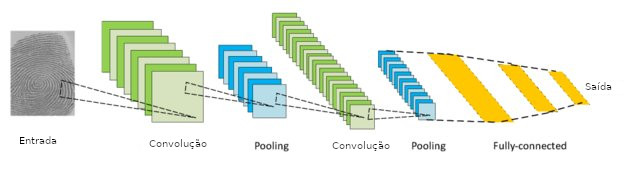
\includegraphics[width=1\linewidth]{recursos/imagens/deep/cnn.jpg}
    \label{cnn:fig:10}

    Fonte: retirada e adaptado de \cite{Minaee2021DeepClassification}.
\end{figure}

Sendo assim, nas próximas seções, fatores que compõem uma rede convolucional serão detalhados, como a camada convolucional (Seção \ref{cnn:conv}), a camada de \textit{pooling} (Seção \ref{cnn:pooling}), fator \textit{dropout} (Seção \ref{cnn:dropout}) e a camada de saída (Seção \ref{cnn:output}) da rede.


\subsection{Camada Convolucional}
\label{cnn:conv}

Na arquitetura das CNNs, a modelagem de cada neurônio presente na camada convolucional envolve a aplicação de um filtro na imagem em análise \citep{ponti2018funciona}. Esses filtros são compostos por pesos e a operação de convolução é categorizada como uma operação linear \citep{Goodfellow2016}, resultando nos chamados mapas de características (\textit{feature maps} em inglês).

É fundamental destacar que entre as camadas convolucionais existem $N$ filtros, cujos parâmetros são definidos de acordo com a natureza do problema em questão, utilizando seus resultados para formar tensores, conforme comentado por \cite{ponti2018funciona}.

A operação de convolução pode ser ilustrada pela Figura \ref{cnn:fig:6}, onde uma imagem de entrada é representada pela matriz de maior escala. Nesse processo, utiliza-se uma janela, conhecida como \textit{kernel}, composta por pesos, que convolui com a matriz de entrada para extrair características específicas da imagem, mantendo a integridade das informações sobre sua disposição espacial.

Essas operações são fundamentais nas CNNs, pois permitem a extração eficiente de características importantes das imagens, o que é crucial para a eficácia e a precisão do processo de aprendizado da rede neural convolucional.

\begin{figure}[H]
    \centering
    \caption{Representação do processo de convolução.}
    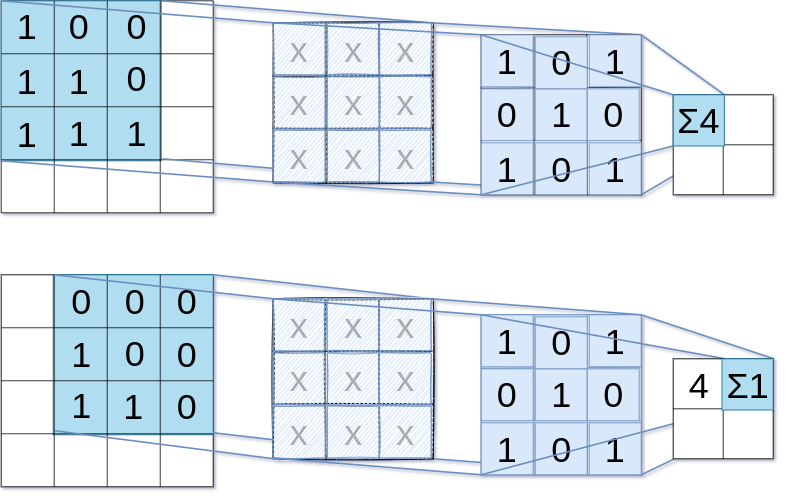
\includegraphics[width=1\linewidth]{recursos/imagens/deep/2d_convolution.png}
    \label{cnn:fig:6}

    Fonte: do próprio autor.
\end{figure}

Ainda na Figura \ref{cnn:fig:6}, é possível observar o processo de deslizamento do \textit{kernel} durante a operação de convolução, resultando em um dos valores presentes na saída. Esse processo é repetido até que toda a imagem seja percorrida, de maneira sequencial da esquerda para a direita e de cima para baixo, movimentando-se através das linhas e colunas.

É crucial ressaltar que a convolução é um processo de média móvel, isto é, implica no cálculo da média ponderada de uma janela específica na imagem, correspondente ao tamanho do \textit{kernel} utilizado. Nesse contexto, o \textit{kernel} define os pesos aplicados aos pontos da janela. Consequentemente, à medida que o \textit{kernel} desliza pela imagem, novas janelas são definidas e suas médias ponderadas são computadas.

Essa abordagem de convolução, com seu deslizamento e cálculo ponderado, é essencial para a extração de informações significativas da imagem, contribuindo para a identificação de padrões relevantes ao longo do processo de aprendizado da rede neural convolucional.


\subsection{Camada de \textit{Pooling}}
\label{cnn:pooling}

Dentro do contexto das camadas de \textit{pooling}, é relevante mencionar que essas camadas são amplamente empregadas nas CNNs com o propósito de reduzir o tempo de treinamento, já que sua função primária é diminuir a dimensionalidade dos mapas de características entre as iterações da rede.

É digno de nota que a adaptação e evolução desses métodos de \textit{pooling} têm recebido crescente atenção na literatura recente \citep{Sabri2020AClassificationb, zafar2022comparison}. Cada modificação busca contribuir para a solução de problemas específicos, evidenciando o constante desenvolvimento dessas técnicas na área de visão computacional e aprendizado profundo.

Ademais, vale ressaltar que na literatura existem diversos modelos de \textit{pooling} que se destacam no uso em redes de aprendizado profundo. Entre eles, destacam-se o \textit{max pooling}, \textit{average pooling}, \textit{median pooling} e \textit{weighted average} \citep{Goodfellow2016}. Há também outros modelos comumente encontrados em redes mais modernas, como o \textit{global average pooling}, \textit{global max pooling} e \textit{astrous spatial pyramid pooling}, principalmente em aplicações de segmentação ou com propostas alternativas. Alguns desses modelos serão discutidos a seguir.

\subsubsection{\textit{Max Pooling}}
\label{cnn:pooling:max_pooling}
Algo que fica muito claro ao observar a Figura \ref{cnn:fig:7}, que dá forma à técnica conhecida como \textit{max pooling}, a qual captura apenas os maiores valores do mapa de características, de acordo com o deslizamento do \textit{kernel}.

\begin{figure}[H]
    \centering
    \caption{\textit{Max pooling}.}
    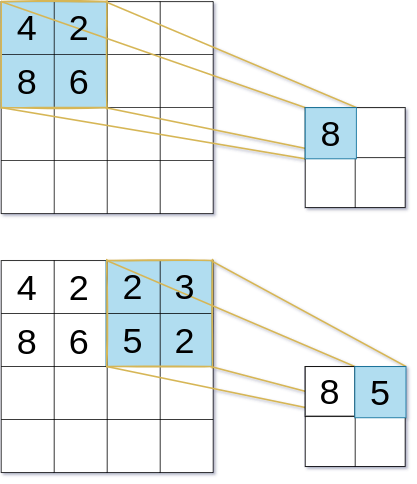
\includegraphics[width=0.5\linewidth]{recursos/imagens/deep/max_pooling.png}
    \label{cnn:fig:7}

    Fonte: do próprio autor.
\end{figure}

\subsubsection{\textit{Average Pooling}}
\label{cnn:pooling:avg_pooling}


\subsubsection{\textit{Global Max Pooling}}
\label{cnn:pooling:global_max_pooling}

até mesmo o \textit{global average pooling}, que reduz o \textit{feature map} em um único valor e é exemplificado por meio da Figura \ref{cnn:fig:8}.

\begin{figure}[H]
    \centering
    \caption{\textit{Global average pooling}.}
    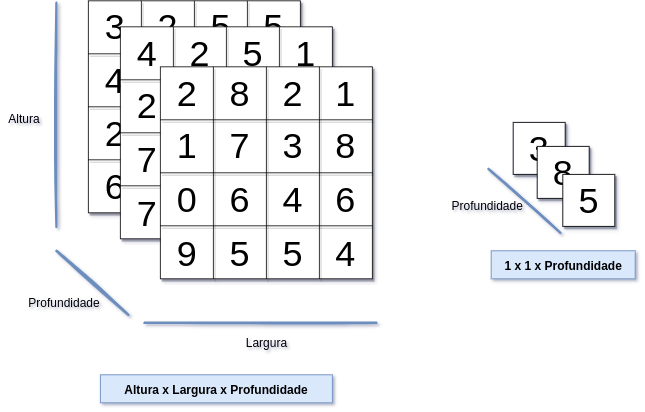
\includegraphics[height=3in]{recursos/imagens/deep/global_average_pooling.png}
    \label{cnn:fig:8}

     Fonte: do próprio autor.
\end{figure}

\subsubsection{\textit{Global Average Pooling}}
\label{cnn:pooling:global_avg_pooling}



\subsubsection{\textit{Atrous Spatial Pyramid Pooling}(ASPP)}
\label{cnn:pooling:aspp}
Basicamente, a abordagem relacionada ao módulo de \textit{Atrous Spatial Pyramid Pooling} (ASPP) \citep{Chen2018} está atrelada às segmentações semânticas \citep{Mohan2020}, sendo que este módulo tem como sua principal vantagem a captura de objetos e contexto úteis da imagem em várias escalas diferentes, haja vista que seu comportamento está atrelado à re-amostragem com diversas taxas de convolução para cada \textit{kernel}, possibilitando, assim, a sondagem de um mapa de características, antes mesmo do processo de convolução, com vários campos de visão \cite{Chen2018}. O exemplo desse módulo pode ser visualizado na Figura \ref{proposal:pcapooling:fig:1}.

\begin{figure}[H]
    \centering
    \caption{Exemplo representativo do ASPP.}
    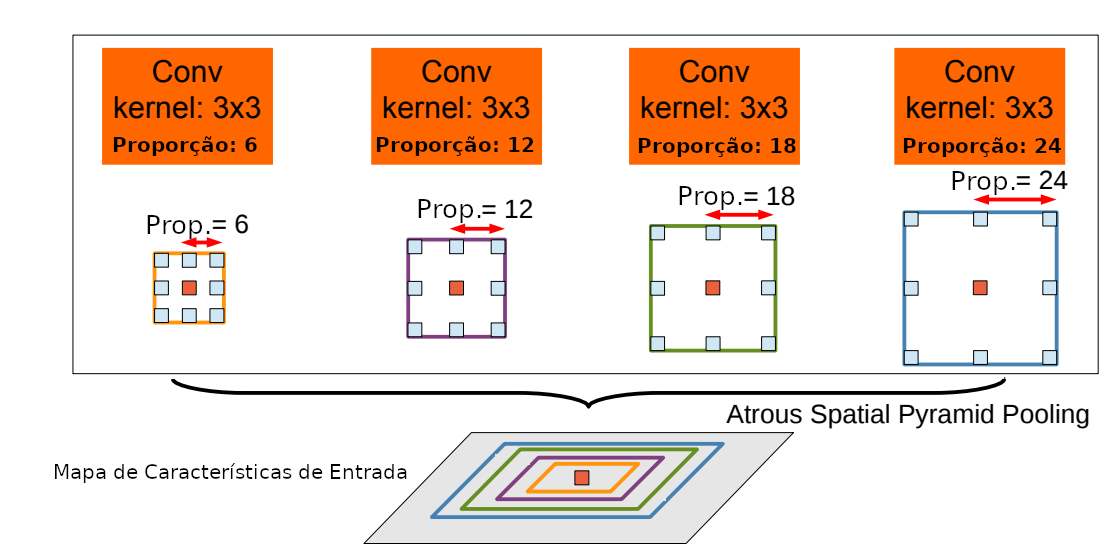
\includegraphics[width=1\textwidth]{recursos/imagens/proposal/aspp.png}
    \label{proposal:pcapooling:fig:1}

    Fonte: retirado e adaptado de \cite{Chen2018}.
\end{figure}

Já quando se trata do módulo de \textit{Pyramid Pooling} \citep{Zhao2017}, vale dizer que este está atrelado à dimensão das características, tendo como principal motivação provar ser um \textit{pooling} de contexto global antes de realizar sua representação \cite{Zhao2017}. Todavia, quando se trata desse modelo de \textit{pooling}, vale dizer que a sua maior vantagem está relacionada à flexibilidade que é cedida às entradas das redes, de modo que torna-se possível realizar entradas com tamanhos variados. O exemplo desse módulo pode ser visualizado na Figura \ref{proposal:pcapooling:fig:2}.

\begin{figure}[H]
    \centering
    \caption{Exemplo representativo do \textit{Pyramid Pooling}.}
    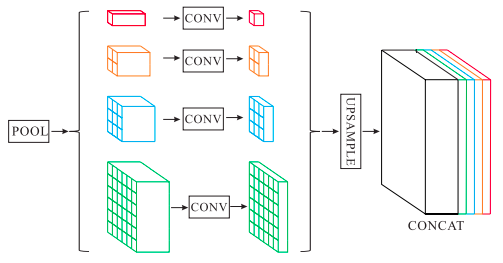
\includegraphics[width=1\textwidth]{recursos/imagens/proposal/pyramidal.png}
    \label{proposal:pcapooling:fig:2}

    Fonte: retirado e adaptado de \cite{Zhao2017}.
\end{figure}

\subsection{\textit{Dropout}}
\label{cnn:dropout}

Dentre as estratégias para mitigar o \textit{overfitting} ,citado na Seção \ref{deep:overunder}, destaca-se a técnica de \textit{dropout} \citep{Goodfellow2016}. Esta técnica, embora não seja aplicada durante a fase de testes, consiste no desligamento aleatório de neurônios em camadas ocultas de uma rede CNN. O propósito do \textit{dropout} é reduzir o viés dos neurônios e aumentar a importância dos neurônios restantes.

O processo de \textit{dropout} é ilustrado na Figura \ref{cnn:fig:9}, mostrando apenas as conexões entre os neurônios restantes, no lado direito da Figura.

\begin{figure}[H]
    \centering
    \caption{Processo de \textit{dropout}.}
    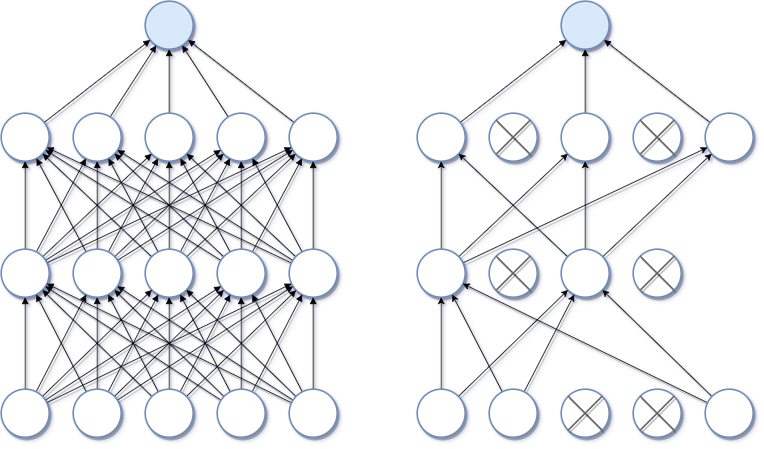
\includegraphics[width=1\linewidth]{recursos/imagens/deep/dropout.png}
    \label{cnn:fig:9}

     Fonte: do próprio autor.
\end{figure}

A técnica de \textit{dropout} é uma estratégia eficaz para regularização em redes neurais, pois ajuda a evitar que a rede se ajuste excessivamente aos dados de treinamento, tornando-a mais capaz de generalizar para dados novos e não vistos durante o treinamento.

\subsection{Camada de Saída}
\label{cnn:output}

Após a composição de várias camadas de convolução, utilizando filtros, e a aplicação de camadas de \textit{pooling}, os modelos de CNN geralmente incluem uma camada de saída, também conhecida como camada densa. Esta camada é fundamental para a determinação das classes identificadas na imagem. Vale destacar que essa camada não tem um impacto significativo no desempenho em relação ao tempo de convergência do modelo, nem interfere no progresso e evolução do processo de treinamento, sendo que o processo de inferência é muito similar ao usado pelas CNNs na Seção \ref{cnn}.

Por fim, para gerar a saída final, é comum utilizar funções de ativação como a Softmax (abordada na Seção \ref{deep:soft}). A aplicação da Softmax permite a identificação da classe de um objeto específico em uma imagem, por exemplo. Essa função de ativação é utilizada para a tarefa de classificação, fornecendo as probabilidades de pertencimento a cada classe no conjunto de dados.


\subsection{Transferência de Aprendizado}
\label{cnn:transfer}

\subsection{Aumento de Dados}
\label{cnn:augment}

\subsection{VGG-16}
\label{cnn:vgg}

\subsection{Considerações Finais do Capítulo}